
\subsection{Reducing the Input Dimension}

The size of input is determined by the dimension of inputs (originally \(16 \times 16\)) and the depth of each pixel (8-bit in the previous design).
A search is done by trying different pair of input dimension and depth and calculating the prediction accuracy using linear regression model, which is actually a lower bound we can achieve.
The result is as \autoref{fig:mnist-shrink}.

It is shown that 

When the input size is shrunk to \(8 \times 8\), the misclassifications rate is 15.96\%, which is slightly worse than our target (over 85\% in accuracy).
However, this is a desirable configuration, which means we can fit an input in precisely 8 bytes.
Thus I believe it is worth sacrificing some accuracy here and getting it back using a more aggressive model.

\begin{figure}[ht!]
    \centering
    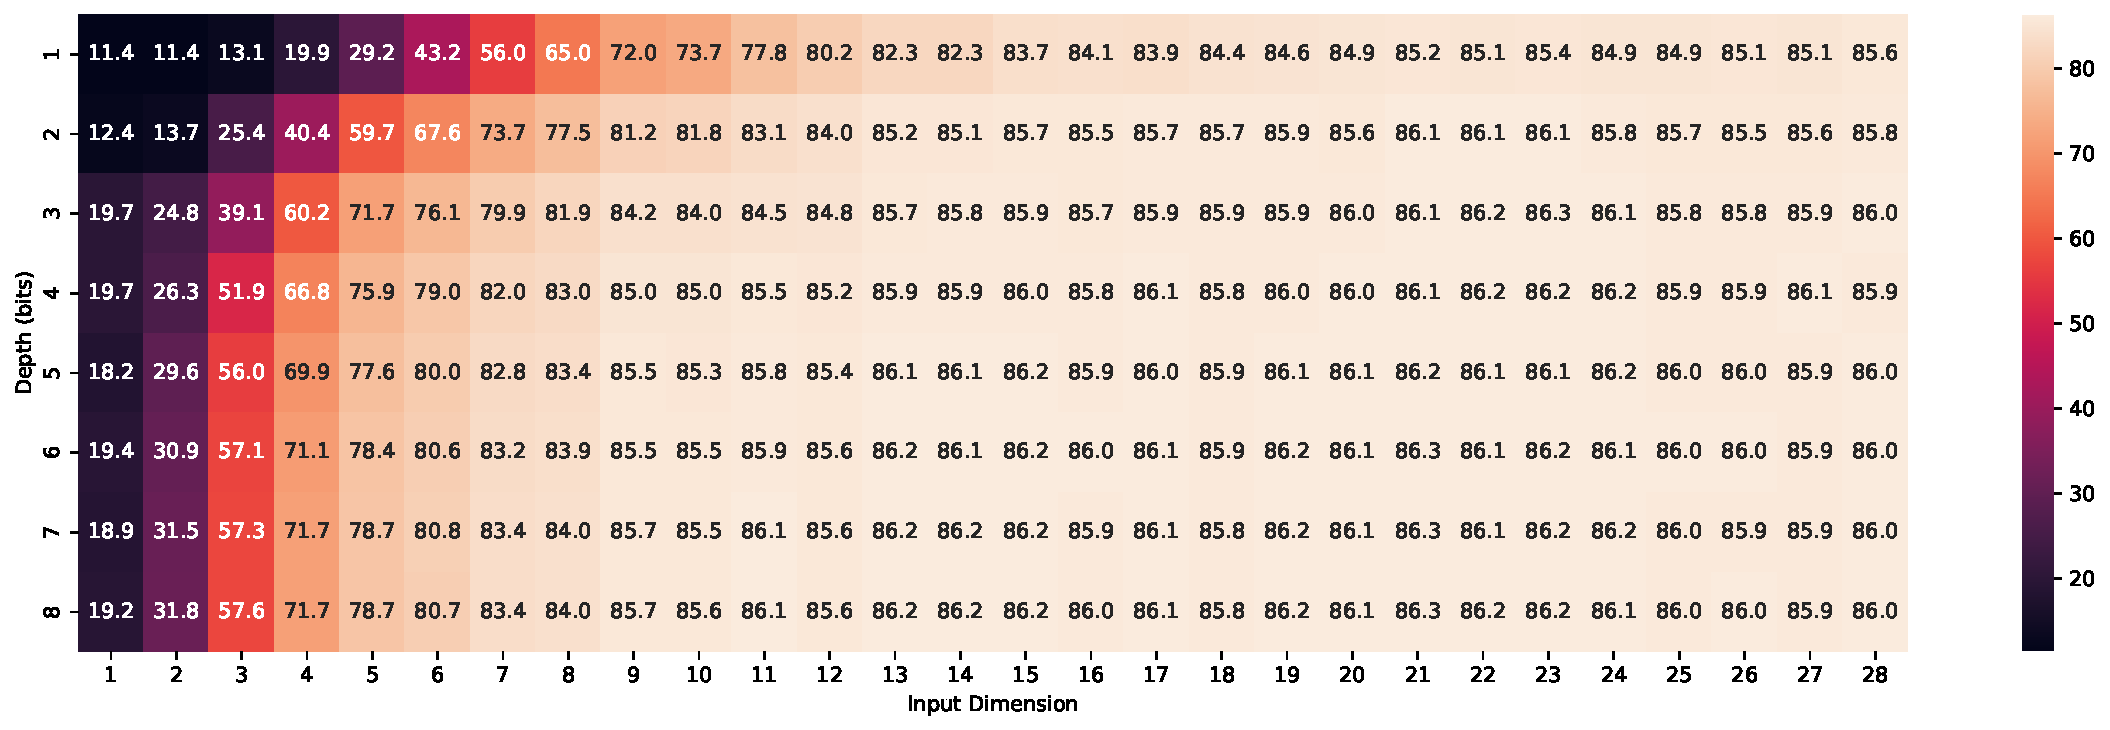
\includegraphics[width=\textwidth]{images/mnist-shrink.pdf}
    \caption{Accuracy of prediction using floating point numbers under different input size}
    \label{fig:mnist-shrink}
\end{figure}

\subsection{Improve Prediction Accuracy}

The accuracy is improve by using a more complex model, which includes a ReLU activated input layer (\(64 \times 16\)), which is unbiased, and a biased output layer (\(16\times 10\)).
Using ReLU with an unbiased input layer, we can refrain from floating point calculation while keep the linear property.

\[
    \mathbf{O} = \operatorname{ReLU}(\mathbf{I} \cdot \mathbf{W_1}) \cdot \mathbf{W_2} + \mathbf{b}
\]

To get a better training result, we add a Softmax layer after the model and use train towards minimized cross entropy loss.
This layer can be removed when predicting on FPGA, which will not affect the final result.

\subsection{Evaluation}

Our design took 4.54 ms to generate the prediction while the CPU used 169.64 ms, which means the FPGA solution achieves a 37.36x speedup against the CPU solution.
The prediction accuracy is 88.18\% on both FPGA and CPU.









% Since we modified the AXI data width, the data width of DMA IP needs to be fixed manually as \autoref{fig:adjust-axi-data-width}.

% \begin{figure}
%     \centering
%     \caption{Adjust AXI data width by re-customizing AXI-DMA IP}
%     \label{fig:adjust-axi-data-width}
%     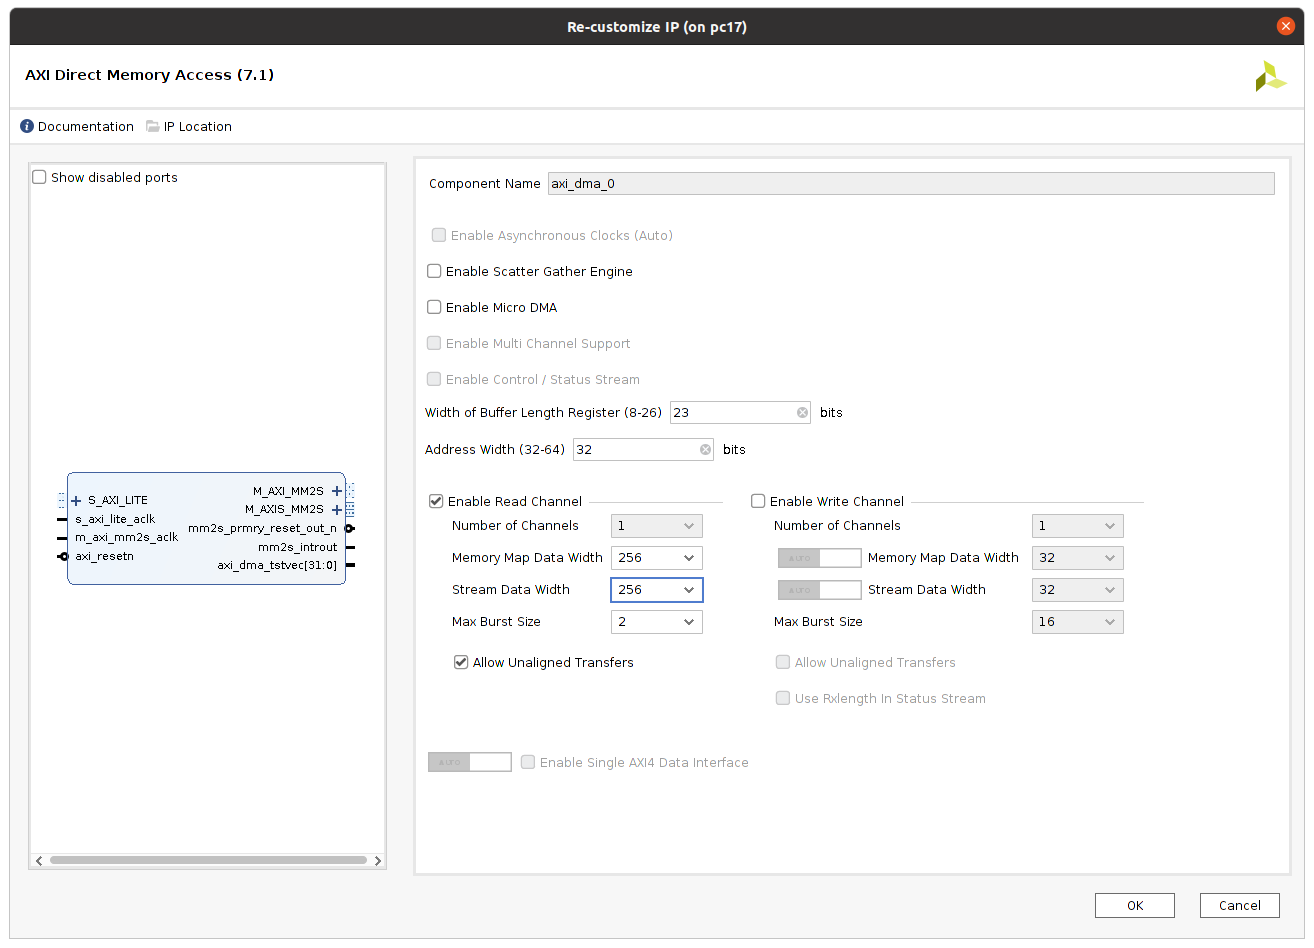
\includegraphics[scale=0.32]{images/adjust-axi-data-width.png}
% \end{figure}










% \subsection{Reduce I/O Latency}

% As we've discussed in \autoref{sec:reflection}, our current design is limited by I/O.
% Thus we seek for reducing the I/O latency, first of all.

% The I/O latency is determined by the number of bits we can transfer per cycle and the number of bits needed to transfer in total.

% \subsubsection{Enhancing a Single AXI Transfer}

% In order to accomodate more data in a single AXI transfer\footnote{
%     \href{https://developer.arm.com/documentation/ihi0051/a/Introduction/About-the-AXI4-Stream-protocol/Stream-terms}{Stream terms}
% }, we need to increase the \texttt{TDATA} width.

% The width in the default design is 64 bits, which took 32 cycles to transfer a single input of 256 bytes.
% By widening the \texttt{TDATA} width to 256 bits, it takes only 8 cycles to transfer the 256 bytes (\autoref{tab:tdata}).

% \begin{table}[ht!]
%     \centering
%     \caption{\texttt{LOAD\_INPUT} latency under different \texttt{TDATA} width}
%     \label{tab:tdata}
%     \begin{tabular}{cccccccc}
%         \toprule
%         \texttt{TDATA} width (bits) & Latency (cycles) & Iteration Latency & Initiation Interval (achieved) & Trip Count & Pipelined \\
%         \midrule
%         64                          & 4096             & 32                & 32                             & 128        & yes       \\
%         128                         & 2048             & 16                & 16                             & 128        & yes       \\
%         256                         & 1024             & 8                 & 8                              & 128        & yes       \\
%         \bottomrule
%     \end{tabular}
% \end{table}
